\documentclass[12pt]{article}

\usepackage[margin=1in]{geometry}
\usepackage{amsmath,amsthm,amssymb}
\usepackage{fancyhdr}
\usepackage[small,compact]{titlesec}
\usepackage{float}

\lhead{Erich Menge}
\chead{\classnameandsection}
\rhead{\homeworktitle}

\pagestyle{fancy}

\newcommand{\sethomeworknumber}[1]{
  \newcommand{\homeworktitle}{Homework #1}
}

\newcommand{\N}{\mathbb{N}}
\newcommand{\Z}{\mathbb{Z}}
\newcommand{\homeworkheader}[1]{
  \title{\vspace{2in}\homeworktitle}
  \author{Erich Menge (X.500: menge053, Student ID: 4624713) \\
  #1}
  \maketitle
  \newpage
}

\newenvironment{problem}[1]{
  \ignorespaces
  \section*{Problem #1}
}{
  \ignorespacesafterend
}

\newenvironment{solution}{
  \ignorespaces
  \subsection*{Solution}
}{
  \ignorespacesafterend
}

\newcommand{\classnameandsection}{CSCI 4011 Formal Languages And Automata Theory Section 3}


\usepackage{graphicx}
\usepackage{pgf}
\usepackage{tikz}
\usepackage{subfigure}
\usetikzlibrary{arrows,automata}

\sethomeworknumber{2}

\begin{document}
\homeworkheader{\classnameandsection}

\begin{problem}{1}
  Do Exercise 1.28 parts c from the book.
  \begin{solution}
    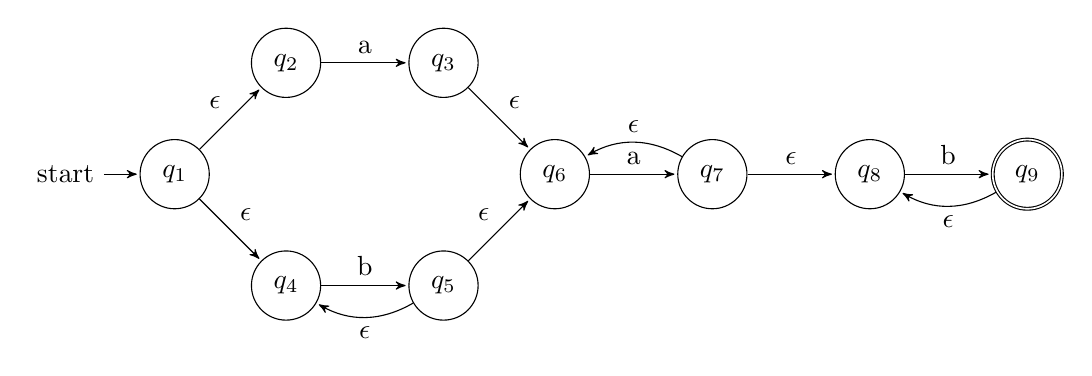
\begin{tikzpicture}[>=stealth',shorten >=1pt,auto,node distance=2cm]
      \node[initial, state] (q1){$q_1$};
      \node[state] [above right of=q1] (q2){$q_2$};
      \node[state] [below right of=q1] (q4){$q_4$};
      \node[state] [right of=q2] (q3){$q_3$};
      \node[state] [right of=q4] (q5){$q_5$};
      \node[state] [below right of=q3] (q6){$q_6$};
      \node[state] [right of=q6] (q7){$q_7$};
      \node[state] [right of=q7] (q8){$q_8$};
      \node[state, accepting] [right of=q8] (q9){$q_9$};

      \path[->]
        (q1)
          edge node{$\epsilon$}(q2)
          edge node{$\epsilon$}(q4)
        (q2)
          edge node{a}(q3)
        (q3)
          edge node{$\epsilon$}(q6)
        (q4)
          edge node{b}(q5)
        (q5)
          edge[bend left] node{$\epsilon$}(q4)
          edge node{$\epsilon$}(q6)
        (q6)
          edge node{a}(q7)
        (q7)
          edge node{$\epsilon$}(q8)
          edge [bend right] node[swap]{$\epsilon$}(q6)
        (q8)
          edge node{b}(q9)
        (q9)
          edge[bend left] node{$\epsilon$}(q8)
      ;

    \end{tikzpicture}

  \end{solution}
\end{problem} \newpage

\begin{problem}{2}
  Do Exercise 1.21 part b from the book.

  \begin{solution}
    \begin{figure}[H]
      \centering
      \caption{Convert NFA to regular expression}
      \subfigure[Step 1 GNFA]{
        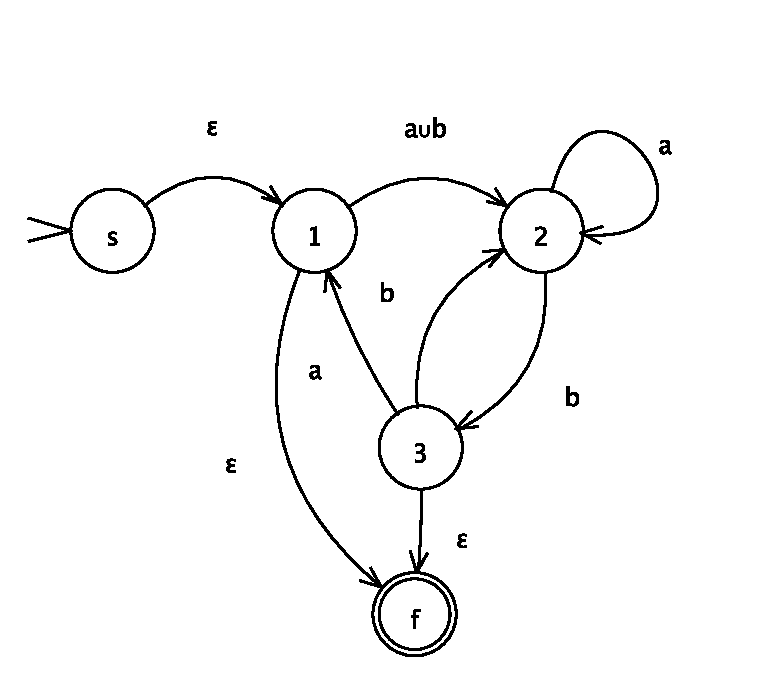
\includegraphics[scale=.6]{1_21_1.eps}
      }
      \subfigure[Step 2 - Remove a state]{
        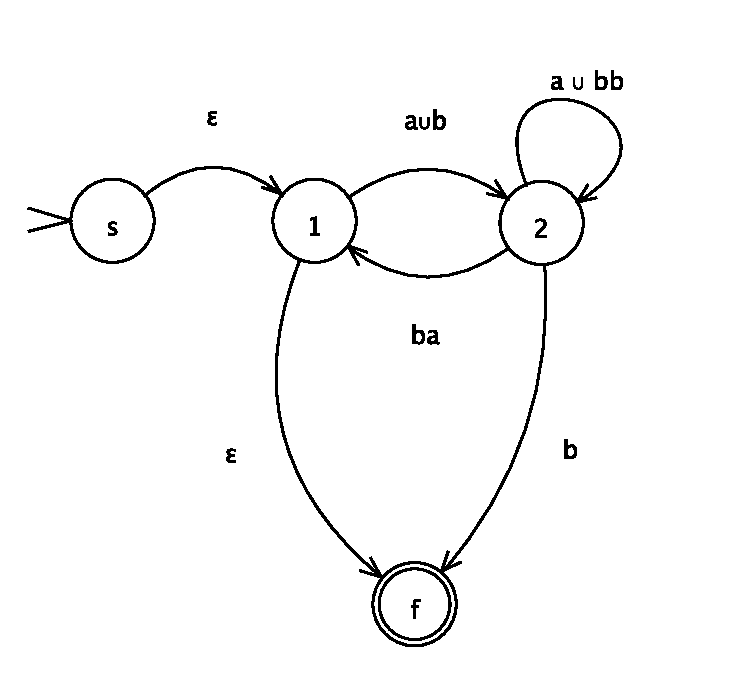
\includegraphics[scale=.6]{1_21_2.eps}
      }
      \subfigure[Step 3 - Remove a state]{
        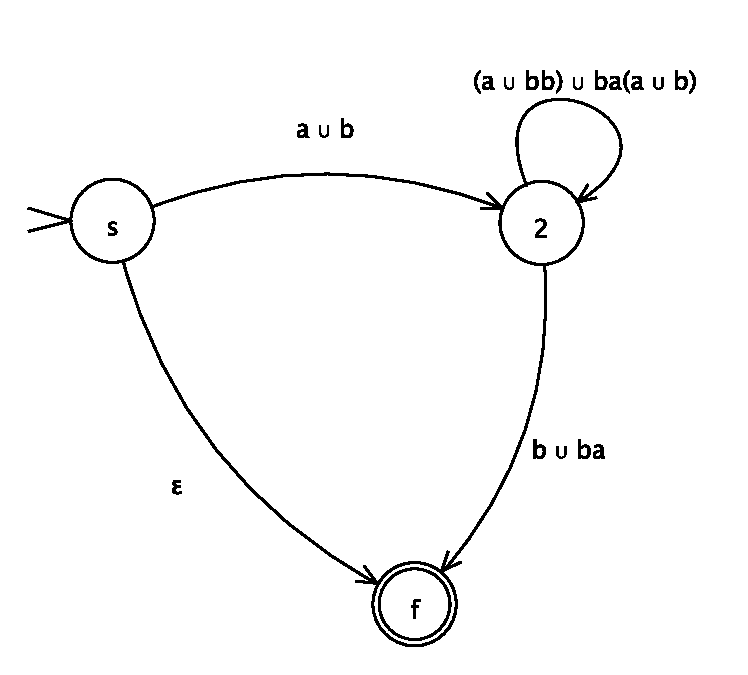
\includegraphics[scale=.6]{1_21_3.eps}
      }
      \subfigure[Step 4 - Only 2 states left]{
        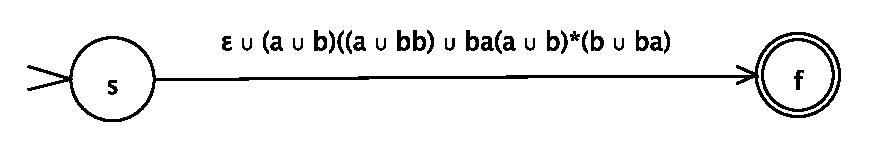
\includegraphics[scale=.6]{1_21_4.eps}
      }
    \end{figure}
  So the resulting regular expression is $ε ∪ (a ∪ b)((a ∪ bb) ∪ ba(a ∪ b)^*(b ∪ ba))$.
  \end{solution}
\end{problem} \newpage

\begin{problem}{3}
  Do Problem 1.41 from the book. The most obvious way to solve this problem is by is by showing how to construct a finite automaton accepting the perfect shuffle of A and B from dfas accepting A and B.

  \begin{solution}
    Let $A = (Q_A, \Sigma_A, \delta_A, q_a, F_A)$ \\
    Let $B = (Q_B, \Sigma_B, \delta_B, q_b, F_B)$ \\

    \noindent Then let $M$ be some machine recognizing the perfect shuffle of $A$ and $B$ where $M$ is defined as a
    5 tuple $(Q, \Sigma, \delta, q, F)$. \\

    \begin{proof}
      If A is regular and B is regular then M can be proved regular by construction: \\

          \noindent $Q = Q_A \times Q_B \times \{ A, B \}$ We have combinations of $Q_A$ and $Q_B$ and symbols representing each machine
          because we will need to ``cycle'' back and forth between the sets of states an even amount of times. \\

          \noindent $\Sigma = \Sigma_A \cup \Sigma_B$ \\

          \noindent $\delta = \delta((Q_{Ai}, Q_{Bi}, A), a) = (\delta_A(Q_{Ai}, a), Q_{Bi}, B)$ and $\delta((Q_{Ai}, Q_{Bi}, B), b) = (Q_{Ai}, \delta_B(q_{bi}, b), A)$ so that the letters of A map to the letters of B, and vice versa, causing a cycling back and forth between the states of each machine. \\

          \noindent $q = (q_a, q_b, A)$ so that the start state requires the first letter to be from machine A. \\

          \noindent $F = F_A \times F_B \times \{ A \}$ so that we end on a state from machine A as we started on it, this means that we have completed an even cycle which is required by definition.
    \end{proof}

    \noindent So this DFA transitions us back and forth between states from A and states from B in order, requiring an
    even cycle so that we start on A and end on A. A perfect shuffle.
  \end{solution}
\end{problem} \newpage

\begin{problem}{4}
  Do Problem 1.46 parts c from the book.
  \begin{solution}
    If $C = \{ w|w \in \{ 0,1 \}^* \text{ is not in a palindrome }\}$ is regular then its complement $\overline{C}$, which contains
    all strings that \underline{are} palindroms, is also regular using closure properties.
    \begin{proof}
      Let $S = 0^p10^p = xyz$ be some string that is a palindrome. \\
      \begin{align*}
        x &= 0^p \\
        y &= 1 \\
        z &= 0^p \\
        |xy| &\le p, |y| > 0
      \end{align*}
      By the Pumping Lemma $0^{p+j}10^p$ should also be in the language of $\overline{C}$, but it violates the definition of
      $\overline{C}$. Therefore $\overline{C}$ must not be regular and by closure properties $C$ is not regular either.
    \end{proof}
  \end{solution}
\end{problem}

\begin{problem}{5}
  Do Problem 1.47 from the book. You may find it useful to use the fact that regular languages are closed under complementation.
\end{problem}

\begin{problem}{6}
  Let $\Sigma$ = \{0,1\}
  \begin{enumerate}
    \item Let A = $\{ 0^ku0^k | k \ge 1$ and $u \in \Sigma^* \}$ Show that A is regular \\
    \item Let B = $\{ 0^k1u0^k | k \ge 1$ and $u \in \Sigma^* \}$. Show that B is not regular.
  \end{enumerate}
\end{problem}

\begin{problem}{7}
  Define the avoids operation on languages A and B to be \\
  \newline\indent avoids(A,B) = $\{ w | w \in$ A and $w$ does not contain any string in B as a substring $\}$ \\
  \newline Prove that the class of regular languages is closed under the avoids operation.
\end{problem}


\end{document}
